\subsection{Briefly outline the main result of time-dependent perturbation theory in a two level system. Explain how this result is related to spectroscopic experiments.}


\paragraph{Toniveausystem:} Toniveausystemet er en måde at beskrive et atom med kun to energiniveauer: Grundtilstanden $\psi_1(\Vec{r}) = \ket{1}$ og den exciterede tilstand $\psi_2(\Vec{r}) = \ket{2}$ med energier på hhv. $E_1$ og $E_2$, som kan være udartede (eng. degenerate). En partikel kan ved interaktion med en foton hoppe mellem disse energiniveauer ved absorption ($\ket{1} \rightarrow \ket{2}$) og stimuleret emission ($\ket{2} \rightarrow \ket{1}$), eller blot hoppe fra $\ket{2} \rightarrow \ket{1}$ grundet spontan emission, hvilket ikke kræver interaktion med en foton.

Til enhver tid kan  partiklens tilstand i toniveausystemet beskrives som en linearkombination af de to tilstande
\begin{align} \label{eq:Q03_TotalBoelgefunktionTidsafhaengig}
    \Psi(\Vec{r},t) &= c_1\ket{1}\exp{-i\omega_1 t} + c_2\ket{2}\exp{-i\omega_2 t} \: ,
\end{align}
hvor $c_j = c_j(t)$ og $\omega_j = E_j/\hbar$ for $j = 1,\,2$, og normalisering kræver at
\begin{align}
    \abs{c_1} + \abs{c_2} &= 1 \: .
\end{align}


\paragraph{Perturbation med oscillerende elektrisk felt:} Udsættes systemet for elektromagnetisk stråling (lys) fra et oscillerende elektrisk felt $\Vec{E} = \Vec{E}_0\cos(\omega t)$ forekommer perturbationen
\begin{align}
    H'(t) &= e\Vec{r} \cdot \Vec{E}_0 \cos(\omega t) \: ,
\end{align}
hvilket tilsvarer energien fra en elektrisk dipol\footnote{Klassisk finder man dipolmomentet som $\Vec{p} = q\Vec{d}$, hvor $q$ er partiklens ladning, og $\Vec{d}$ dens afstand fra massemidtpunktet. Derved findes den potentielle energi for en elektron $U = -\Vec{p}\cdot\Vec{E}$, hvorved potentialet bliver $V = +e\Vec{r}\cdot\Vec{E}$, hvor $e$ er elementarladningen.} $-e\Vec{r}$ i det elektriske felt, hvor $\Vec{r}$ er elektronens placering relativ til atomets massemidtpunkt. Det er antaget, at dipolmomentet kun opstår grundet én enkelt partikel, men dette kan generaliseres ved at summere over alle elektronerne i et atom.

Denne interaktion med lys blander tilstandene med energier $E_1$ og $E_2$. Indsættes \cref{eq:Q03_TotalBoelgefunktionTidsafhaengig} i den tidsafhængige Schrödingerligning fås
\begin{align}
    i\Dot{c}_1 &= \Omega \cos(\omega t) \exp{-i\omega_0 t} c_2 \: , \label{eq:Q03_CoupledDifferentialEquationsForC1AndC2_C1} \\
    i\Dot{c}_2 &= \Omega^* \cos(\omega t) \exp{i\omega_0 t} c_1 \: , \label{eq:Q03_CoupledDifferentialEquationsForC1AndC2_C2}
\end{align}
hvor $\omega = (E-2 - E_1)/\hbar = \Delta E / \hbar$, og \emph{Rabifrekvensen} $\Omega$ er defineret ved
\begin{align}
    \Omega &= \frac{\bra{1}e\Vec{r}\cdot\Vec{E}_0\ket{2}}{\hbar} = \frac{e}{\hbar} \int \psi_1^* \Vec{\Vec{r}} \cdot \Vec{E}_0 \psi_2(\Vec{r}) \: \text{d}^3\Vec{r} \: .
\end{align}
Grundet \emph{dipolapproksimationen} vil det elektriske felt have en stort set uniform amplitude over hele den atomare bølgefunktion, hvorfor vi antager amplituden $|\Vec{E}_0|$ konstant og må derfor flytte denne udenfor integralet.\footnote{Dipolapproksimationen holder så længe, at lysets bølgelængde er større end atomet, $\lambda \gg a_0$.} Lader vi nu lyset være lineært polariseret lang $x$-aksen, $\Vec{E} = |\Vec{E}_0|\Hat{e}_x\cos(\omega t)$, får vi Rabifrekvensen
\begin{align}
    \Omega &= \frac{e\bra{1}x\ket{2}\abs{\Vec{E}_0}}{\hbar} \: .
\end{align}


\paragraph{Roterende bølge-approksimation:} For at løse de koblede differentialligninger for $c_1(t)$ og $c_2(t)$ (\cref{eq:Q03_CoupledDifferentialEquationsForC1AndC2_C1,eq:Q03_CoupledDifferentialEquationsForC1AndC2_C2}) er det nødvendigt at lave endnu en antagelse. Vi antager, at at hele populationen starter i grundtilstanden $\ket{1}$, således at $c_1(0) = 1$ og $c_2(0) = 0$, hvilket, når \cref{eq:Q03_CoupledDifferentialEquationsForC1AndC2_C1,eq:Q03_CoupledDifferentialEquationsForC1AndC2_C2} er integreret, giver
\begin{align}
    c_1(t) &= 1 \: , \label{eq:Q03_UdtrykForC1(t)EfterAntagelseOmPopulation}\\
    c_2(t) &= \frac{\Omega^*}{2} \left\{\frac{1 - \exp{i(\omega_0 + \omega)t}}{\omega_0 + \omega} + \frac{1 - \exp{i(\omega_0 - \omega)t}}{\omega_0 - \omega}\right\} \: , \label{eq:Q03_UdtrykForC2(t)EfterAntagelseOmPopulation}
\end{align}
hvilket giver en fornuftig førsteordens approksimation, mens $c_2(t)$ forbliver lille. Vi interresserer os kun for de tilfælde, hvor lyset har en frekvens nær atomets ræsonansfrekvens -- da det kun er i disse tilfælde, at partiklerne i toniveausystemet vil interagere med lyset -- således at afvigelsen (eng. the detuning) er lille, $|\omega_0 - \omega| \ll \omega_0$, hvorved $\omega_0 + \omega \simeq 2\omega_0$. Vi kan derfor negligere det første led i \cref{eq:Q03_UdtrykForC2(t)EfterAntagelseOmPopulation}, da dette indeholder $\omega_0 + \omega$ i nævneren. Dette kaldes \emph{roterende bølge-approksimationen}\footnote{Roterende bølge-approksimation (eng. rotating-wave approximation) er, at $(\omega + \omega_0)t$ oscillerer meget hurtigt, hvorfor dette i gennesnit bliver $0$ over en fornuftig interkationstid.}. Fra denne approksimation bliver sandsynligheden for at finde elektronen i den exciterede tilstand
\begin{align}
    \abs{c_2(t)}^2 &= \abs{\Omega \dfrac{\sin\left(\dfrac{\omega_0 - \omega}{2}t\right)}{\omega_0 - \omega}} \: ,
\end{align}
hvilket kan beskrives ved $x = (\omega_0 - \omega)t/2$,
\begin{align} \label{eq:Q03_ExcitationProbabilityFunction}
    \abs{c_2(t)}^2 &= \frac{1}{4}\abs{\Omega}^2t^2\frac{\sin^2(x)}{x^2} = \frac{1}{4}\abs{\Omega}^2t^2\mathrm{sinc}^2(x) \: .
\end{align}
Sandsynlighedsfunktionen er afbilledet på \cref{fig:Q03_ExcitationProbabilityFunction}. Her kan man tydeligt se, at der er størst sandsynlighed for at observere systemet i den exciterede tilstand, når lysets frekvens $\omega$ er tæt ved atomets ræsonansfrekvens $\omega_0$, hvor amplituden også hurtigt aftager ved overtonerne, grundet den $x^{-2}$-ledet. Det kan også ses, at som tiden går, så vil sandsynligheden sprede sig ud og dermed aftage.

\begin{figure}[!h]
    \centering
    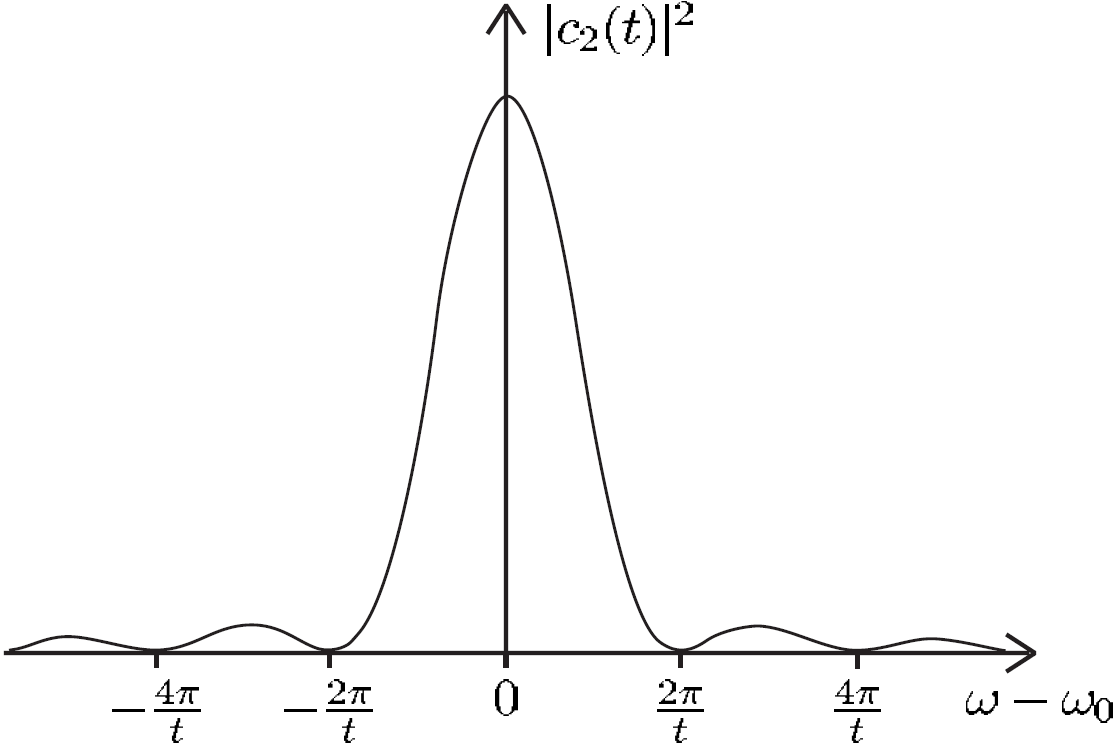
\includegraphics[width=0.75\textwidth]{Q03/images/ExcitationProbabilityFunction.PNG}
    \caption{Excitationssandsynligheden er størst idet, at det indsendte lys har en frekvens $\omega$, som stort set matcher atomets ræsonansfrekvens $\omega_0$. Functionens bredde er invers proportional med tiden, hvorfor sandsynligheden vil falde som tiden går.}
    \label{fig:Q03_ExcitationProbabilityFunction}
\end{figure}


\paragraph{Resultatets sammenhæng med spektroskopiske eksperimenter:} \ldots